\documentclass[fleqn, a4paper, 8pt, twoside]{amsart}
\usepackage{exsheets} %question and solution environments
\usepackage{amsmath, amssymb, amsthm} %standard AMS packages
\usepackage{esint} %integral signs
%\usepackage{marginnote} %marginnotes
\usepackage{gensymb} %miscellaneous symbols
\usepackage{commath} %differential symbols
\usepackage{xcolor} %colours
\usepackage{cancel} %cancelling terms
\usepackage[free-standing-units]{siunitx} %formatting units
\usepackage{tikz, pgfplots} %diagrams
	\usetikzlibrary{calc, hobby, patterns, intersections, angles, quotes, spy}
%\usepackage{graphicx} %inserting graphics
%\usepackage{epstopdf} %converting and inserting eps graphics
\usepackage{hyperref} %hyperlinks
\usepackage{datetime} %date and time
%\usepackage{ulem} %underline for \emph{}
\usepackage{xfrac, lmodern} %inline fractions
\usepackage{enumerate, enumitem} %numbered lists
\usepackage{float} %inserting floats
\usepackage[american voltages]{circuitikz} %circuit diagrams
\usepackage{pdflscape}
\usepackage{setspace}
\usepackage{microtype}
\usepackage[extreme]{savetrees}
\usepackage{multicol}
\usepackage{titlesec}

\titleformat{\part}
	{\titlerule \vspace{0.2ex} \titlerule \vspace{.8ex} \normalfont \bf \huge}{\thepart}{1em}{}[\titlerule \vspace{0.2ex} \titlerule]
\titleformat{\section}
	{\normalfont \bf \LARGE}{\thesection}{1em}{}
\titleformat{\subsection}
	{\normalfont \bf \Large}{\thesubsection}{1em}{}

\newcommand\numberthis{\addtocounter{equation}{1}\tag{\theequation}} %adds numbers to specific equations in non-numbered list of equations

\newcommand{\AxisRotator}[1][rotate=0]{
	\tikz [x=0.25cm,y=0.60cm,line width=.2ex,-stealth,#1] \draw (0,0) arc (-150:150:1 and 1);%
} %rotation symbols on axes

\theoremstyle{definition}
\newtheorem{example}{Example}
\newtheorem{definition}{Definition}

\theoremstyle{theorem}
\newtheorem{theorem}{Theorem}
\newtheorem{law}{Law}

\newcommand{\curl}{\mathrm{curl\,}}

\newcommand{\divergence}{\mathrm{div\,}}

\makeatletter
\@addtoreset{section}{part} %resets section numbers in new part
\makeatother

\newcommand\blfootnote[1]{%
	\begingroup
	\renewcommand\thefootnote{}\footnote{#1}%
	\addtocounter{footnote}{-1}%
	\endgroup
}

\SetupExSheets{solution/print = true} %prints all solutions by default

%opening
\title{\Huge Physics 2}
\author{Aakash Jog}
\date{\formatdate{26}{6}{2015}}

\begin{document}

\maketitle
%\setlength{\mathindent}{0pt}

\begin{multicols}{2}

\begin{spacing}{0.6}

\part{Electrostatics}

\section{Coulomb's Law}

\begin{law}[Coulomb's Law]
	\begin{align*}
		\overrightarrow{F_{2 1}} &= \frac{1}{4 \pi \varepsilon_0} \frac{q_1 q_2}{{r_{1 2}}^2} \hat{r_{1 2}}
	\end{align*}
	\label{Coulomb's_Law}
\end{law}

\section{Electric Field}

\begin{definition}[Electric field]
	The electric field at a point in space is the electric force felt by a charge of 1 \si{\coulomb} had it been kept there.
\end{definition}

\subsection{Standard Electric Fields}

\begin{tabular}{m{0.4\columnwidth} m{0.4\columnwidth}}
	Point charge & $\frac{q}{4 \pi \varepsilon_0 r^2}$\\
	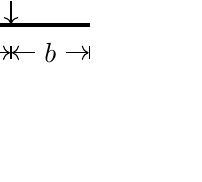
\begin{tikzpicture}
		\def\a{0.8};
		\def\b{1};
		\def\z{1};

		\draw[ultra thick] (-\a,0) -- (\b,0);

		\begin{scope}[yshift = -10, |<->|]
			\draw (0,0) -- (-\a,0) node [midway, fill = white] {$a$};
			\draw (0,0) -- (\b,0) node [midway, fill = white] {$b$};
		\end{scope}
		
		\draw[|<->|] (0,0) -- (0,\z) node [midway, fill = white] {$z$};
	\end{tikzpicture}
	&
	$\frac{\lambda}{4 \pi \varepsilon_0 z} \left( \frac{b}{\sqrt{z^2 + b^2}} + \frac{a}{\sqrt{z^2 + a^2}} \right)$ in the direction perpendicular to the rod\\
	Infinite line of charge & $\frac{\lambda}{2 \pi \varepsilon_0 r}$\\
	Ring of charge & $\frac{\lambda R z}{2 \varepsilon_0 \left( z^2 + R^2 \right)^{\sfrac{3}{2}}}$\\
	Disk of charge & $\frac{\sigma}{2 \varepsilon_0} \left( 1 - \frac{x}{\sqrt{z^2 + R^2}} \right)$\\
	Infinite plane of charge & $\frac{\sigma}{2 \varepsilon_0}$\\
\end{tabular}

\subsection{Capacitors}

\begin{definition}[Capacitance]
	\begin{align*}
		C &= \frac{Q}{V}
	\end{align*}
\end{definition}

\begin{theorem}
	\begin{align*}
		E &= \frac{\sigma}{2 \varepsilon_0}\\
		C &= \frac{A \varepsilon_0}{d}
	\end{align*}
\end{theorem}

\section{Electric Dipoles}

\begin{definition}[Dipole moment]
	If two charges $q$ and $-q$ are separated by a distance $d$, the dipole moment is defined as
	\begin{equation*}
		\overrightarrow{P} = q \cdot \overrightarrow{d}
	\end{equation*}
	where $\overrightarrow{d}$ is the vector of length $d$ pointing from $-q$ to $q$.
\end{definition}

\begin{theorem}
	The electric field at an equatorial point with respect to a dipole of moment $\overrightarrow{P} = q \overrightarrow{d}$ is
	\begin{align*}
		\overrightarrow{E} &= - \frac{1}{4 \pi \varepsilon_0} \frac{\overrightarrow{P}}{\left( \left( \frac{d}{2} \right)^2 + x^2 \right)^{\sfrac{3}{2}}}
	\end{align*}
\end{theorem}

\section{Gauss' Law}

\begin{definition}[Electric flux]
	Electric flux is defined as the dot product of the electric field passing through a surface, and the area vector of the surface.
	\begin{equation*}
		\Phi = \overrightarrow{E} \cdot \overrightarrow{A}
	\end{equation*}
	where the magnitude of the area vector is proportional to the area of the surface and the direction is perpendicular to the surface.
\end{definition}

\begin{law}[Gauss' Law]
	\begin{equation*}
		\oiint \overrightarrow{E} \cdot \overrightarrow{\dif A} = \frac{Q_{\textnormal{inside}}}{\varepsilon_0}
	\end{equation*}
	\label{Gauss'_Law}
\end{law}

\begin{question}
	A metal sphere of radius $R$ carries a total charge $Q$.
	What is the force of repulsion between the ``northern'' hemisphere and the ``southern'' hemisphere?
\end{question}

\begin{solution}
	\begin{align*}
		E_{\textnormal{northern hemisphere}} &= \frac{1}{2} \frac{Q}{4 \pi \varepsilon_0 R^2}
	\end{align*}
	Due to the symmetry of the sphere, the components of the force of all elemental charges, in the direction of the north-south axis add up, and all other components cancel out.\\
	Therefore,
	\begin{align*}
		F & = \int\limits_{0}^{\frac{\pi}{2}} \int\limits_{0}^{2 \pi} E_{\textnormal{northern hemisphere}} \sigma R^2 \dif \varphi \sin(\theta) \cos(\theta) \dif \theta                                                       \\
                  & = \int\limits_{0}^{\frac{\pi}{2}} \int\limits_{0}^{2 \pi} \frac{1}{2} \cdot \frac{1}{4 \pi \varepsilon_0} \cdot \frac{Q}{R^2} \cdot \frac{Q}{4 \pi R^2} R^2 \sin(\theta) \cos(\theta) \dif \varphi \dif \theta \\
                  & = \int\limits_{0}^{\frac{\pi}{2}} \int\limits_{0}^{2 \pi} \frac{1}{2 \pi \varepsilon_0} \left( \frac{Q}{4 \pi R} \right)^2 \sin(\theta) \cos(\theta) \dif \varphi \dif \theta                                    \\
                  & = \int\limits_{0}^{2 \pi} \frac{1}{2 \pi \varepsilon_0} \left( \frac{Q}{4 \pi R} \right)^2                                                                                                                        \\
                  & = \frac{1}{2 \pi \varepsilon_0} \left( \frac{Q}{4 \pi R} \right)^2                                                                                                                                                \\
                  & = \frac{Q^2}{32 \pi^2 \varepsilon_0 R^2}
	\end{align*}
\end{solution}

\section{Electric Potential}

\begin{definition}[Electrical Potential]
	The electric potential due to a point charge $q$ is
	\begin{align*}
		\varphi \left( \overrightarrow{r} \right) &= \frac{1}{4 \pi \varepsilon_0} \frac{q}{r} + c
	\end{align*}
\end{definition}

If a charge $q$ in moved from point $\textnormal{A}$ to $\textnormal{B}$,
\begin{align*}
	W_{\textnormal{\textnormal{A}} \to \textnormal{B}} &= \int\limits_{\overrightarrow{r_{\textnormal{A}}}}^{\overrightarrow{r_{\textnormal{B}}}} \overrightarrow{E} \cdot \dif \overrightarrow{r}\\
	&= \int\limits_{r_{\textnormal{A}}}^{r_{\textnormal{B}}} \frac{1}{4 \pi \varepsilon_0} \frac{q}{r^2} \dif r\\
	&= \left. - \frac{1}{4 \pi \varepsilon_0} \frac{q}{r} \right|_{r_{\textnormal{A}}}^{r_{\textnormal{B}}}\\
	&= \frac{1}{4 \pi \varepsilon_0} \frac{q}{r_{\textnormal{A}}} - \frac{1}{4 \pi \varepsilon_0} \frac{q}{r_{\textnormal{B}}}
\end{align*}

Therefore,
\begin{align*}
	W_{\textnormal{A} \to \textnormal{B}} &= \varphi \left( \overrightarrow{r_A} \right) - \varphi \left( \overrightarrow{r_B} \right)\\
	\therefore \varphi \left( \overrightarrow{r_B} - \overrightarrow{r_A} \right) &= - \int\limits_{\overrightarrow{r_A}}^{\overrightarrow{r_B}} \overrightarrow{E} \cdot \dif \overrightarrow{r}
\end{align*}

\subsection{Standard Electric Potentials}

%~\\
\begin{tabular}{m{0.4\columnwidth} m{0.4\columnwidth}}
	Point charge & $\frac{q}{4 \pi \varepsilon_0 r}$\\
	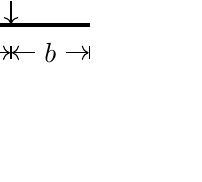
\begin{tikzpicture}
		\def\a{0.8};
		\def\b{1};
		\def\z{1};

		\draw[ultra thick] (-\a,0) -- (\b,0);

		\begin{scope}[yshift = -10, |<->|]
			\draw (0,0) -- (-\a,0) node [midway, fill = white] {$a$};
			\draw (0,0) -- (\b,0) node [midway, fill = white] {$b$};
		\end{scope}
		
		\draw[|<->|] (0,0) -- (0,\z) node [midway, fill = white] {$z$};
	\end{tikzpicture}
	&
	$\frac{\lambda}{4 \pi \varepsilon_0} \ln \left( \frac{b + \sqrt{b^2 + z^2}}{a + \sqrt{a^2 + z^2}} \right)$\\
	Ring of charge & $\frac{\lambda r}{2 \varepsilon_0 \sqrt{r^2 + z^2}}$\\
	Disk of charge & $\frac{\sigma}{2 \varepsilon_0} \left( \sqrt{z^2 + r^2} - z \right)$\\
\end{tabular}

\begin{question}
	Find the electric potential due to an infinite line of charge.
\end{question}

\begin{solution}
	For an infinite line of charge, the charge at infinity is not zero.
	Therefore, it is wrong to assume that the electric potential at infinity is zero.
	Therefore, the result for a finite line of charge cannot be used to find the potential due to an infinite line of charge.\\
	Therefore, the potential needs to be calculated using the electric field.
	\begin{align*}
		\varphi(r) - \varphi(r_0) &= -\int\limits_{r_0}^{r} \overrightarrow{E} \cdot \dif \overrightarrow{r}\\
		&= - \int\limits_{r_0}^{r} E \dif r\\
		&= - \int\limits_{r_0}^{r} \frac{\lambda}{2 \pi \varepsilon_0 r} \dif r\\
		&= \left. - \frac{\lambda}{2 \pi \varepsilon_0} \ln r \right|_{r_0}^{r}\\
		&= \frac{\lambda}{2 \pi \varepsilon_0} (\ln r_0 - \ln r)\\
		\therefore \varphi(r) &= \varphi(r_0) + \frac{\lambda}{2 \pi \varepsilon_0} (\ln r_0 - \ln r)
	\end{align*}
\end{solution}

\begin{question}
	An inverted hemispherical bowl of radius $R$ is carrying a uniform surface charge density $\sigma$.
	Find the potential difference between the ``north pole'' and the center.
\end{question}

\begin{solution}
	If the hemispherical shell was complete, the potential at the centre would be
	\begin{align*}
		\varphi_{\textnormal{full sphere}} &= \frac{1}{4 \pi \varepsilon_0} \frac{Q}{R}\\
		&= \frac{1}{4 \pi \varepsilon_0} \frac{\sigma \cdot 4 \pi R^2}{R}\\
		&= \frac{\sigma R}{\varepsilon_0}
	\end{align*}
	The potential at the centre due to the hemispherical shell is half of that due to the entire shell.\\
	Therefore,
	\begin{align*}
		\varphi_{\textnormal{centre}} &= \frac{1}{2} \left( \frac{1}{4 \pi \varepsilon_0} \frac{\sigma \cdot 2 \pi R^2}{R} \right)\\
		&= \frac{\sigma R}{2 \varepsilon_0}
	\end{align*}
	Consider an elemental ring of radius $r$ at height $z$ from the pole.\\
	Therefore,
	\begin{align*}
		\dif \varphi_{\textnormal{pole}} &= \frac{1}{4 \pi \varepsilon_0} \frac{\sigma \cdot 2 \pi r \dif r}{\sqrt{r^2 + z^2}}\\
		\therefore \varphi_{\textnormal{pole}} &= \frac{\sigma}{2 \varepsilon_0} \int\limits_{0}^{R} \frac{r \dif r}{\sqrt{r^2 + z^2}}\\
		&= \frac{\sigma R}{\sqrt{2} \varepsilon_0}
	\end{align*}
	Therefore,
	\begin{align*}
		\varphi_{\textnormal{pole}} - \varphi_{\textnormal{centre}} &= \frac{\sigma R}{\varepsilon_0} - \frac{\sigma R}{\sqrt{2} - \varepsilon_0}\\
		&= \frac{\sigma R}{\varepsilon_0} \left( \sqrt{2} - 1 \right)
	\end{align*}
\end{solution}

\begin{question}
	A conical surface (an empty ice-cream cone) carries a uniform surface charge $\sigma$.
	The height of the cone is $h$, as is the radius of the top.
	Find the potential difference between points $\mathrm{a}$ (the vertex) and $\mathrm{b}$ (the centre of the top).
\end{question}

\begin{solution}
	\begin{figure}[H]
		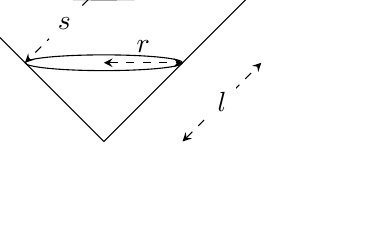
\begin{tikzpicture}
			\def\H{2};
			\def\R{2};
			\def\h{1};
			\def\r{1};
			
			\coordinate (apex) at (0,0);
			\coordinate (base centre) at (0,\H);
			\coordinate (elemental ring centre) at (0,\h);
			
			\draw (base centre) circle [x radius = \R, y radius = 0.1*\R];
			\draw ($ (base centre) + (-\H,0) $) -- (apex);
			\draw ($ (base centre) + (\H,0) $) -- (apex);
			
			\draw (elemental ring centre) circle [x radius = \r, y radius = 0.1*\r];
			
			\begin{scope}[dashed, stealth-stealth]
				\draw (base centre) -- ++(\R,0) node [midway, above] {$h$};
				\draw (elemental ring centre) -- ++(\r,0) node [midway, above] {$r$};
				\draw ($ (apex) + (1,0) $) -- ($ (elemental ring centre) + (\r,0) + (1,0) $) node [midway, fill = white] {$l$};
				\draw (base centre) -- ($ (elemental ring centre) + (-\r,0) $) node [midway, fill = white] {$s$};
			\end{scope}
		\end{tikzpicture}
	\end{figure}
	Consider an elemental ring of radius $r$ and thickness $\dif r$ as shown.\\
	Let $s$ be the distance from the centre of the base to any point on the elemental ring.\\
	Therefore,
	\begin{align*}
		\varphi(a) &= \int \dfrac{k \dif q}{l}\\
		&= \int\limits_{0}^{\sqrt{2} h} \dfrac{k \sigma \cdot 2 \pi r}{l} \dif l\\
		&= \int\limits_{0}^{\sqrt{2} h} \dfrac{2 k \sigma \pi r}{\sqrt{2} r} \dif l\\
		&= \dfrac{2 k \sigma \pi}{\sqrt{2}} \cdot \sqrt{2} h\\
		&= \dfrac{\sigma h}{2 \varepsilon_0}
	\end{align*}
	\begin{align*}
		\varphi(b) &= \int \dfrac{k \dif q}{s}\\
		&= \int\limits_{0}^{\sqrt{2} h} \dfrac{k \sigma \cdot 2 \pi r}{\sqrt{h^2 + l^2 - \sqrt{2} h l}} \dif l\\
		&= \left. \dfrac{2 k \sigma \pi}{\sqrt{2}} \left( \sqrt{h^2 + l^2 - \sqrt{2} h l} \right) \right|_{0}^{\sqrt{2}}\\
		&\quad + \left. \dfrac{2 k \sigma \pi}{\sqrt{2}} \left( \dfrac{h}{\sqrt{2}} \ln \left( 2 \sqrt{h^2 + l^2 - \sqrt{2} h l} + 2 l - \sqrt{2} h \right) \right) \right|_{0}^{\sqrt{2}} \\
		&= \dfrac{\sigma h}{4 \varepsilon_0} \ln \left( 3 + 2 \sqrt{2} \right)\\
		&= \dfrac{\sigma h}{2 \varepsilon_0} \ln \left( 1 + \sqrt{2} \right)
	\end{align*}
	Therefore,
	\begin{align*}
		\varphi(a) - \varphi(b) &= \dfrac{\sigma h}{2 \varepsilon_0} \left( 1 - \ln \left( 1 + \sqrt{2} \right) \right)
	\end{align*}
\end{solution}

\section{Electrical Potential Energy}

\begin{question}
	Three charges, $q$, $-4q$, $2q$ are placed on the vertices of an equilateral triangle of side $a$. Find the energy in the system.
\end{question}

\begin{solution}
	The energy in the system is the amount of energy required to build the system by bringing each of the charges from infinity to its position, one by one.\\
	Let the positions of $q$, $2q$ and $-4q$ be A, B and C respectively.\\
	The energy required to bring the first charge, $q$, from infinity to A is zero, as there are no forces acting on it.\\
	The energy required to bring the second charge, $2q$, from infinity to B is 
	\begin{align*}
		U_{2q} &= - \int\limits_{\infty}^{\overrightarrow{r_\textnormal{B}}} \overrightarrow{F} \cdot \dif \overrightarrow{r}\\
		&= - \int\limits_{\infty}^{\overrightarrow{r_\textnormal{B}}} (2q) \cdot \overrightarrow{E} \cdot \dif \overrightarrow{r}\\
		&= - (2q) \int\limits_{\infty}^{\overrightarrow{r_\textnormal{B}}} \overrightarrow{E} \cdot \dif \overrightarrow{r}\\
		&= (2q) \left( \varphi(\textnormal{B}) - \varphi(\infty) \right)\\
		&= (2q) \cdot \varphi(\textnormal{B})
	\end{align*}
	where $\varphi(\textnormal{B})$ is potential at point B due to the existing charges, i.e. $q$.
	Similarly, the energy required to bring the third charge, $-4q$, from infinity to C is $(-4q) \cdot \varphi(\textnormal{C})$, where $\varphi(\textnormal{C})$ is the potential at point C due to the existing charges, i.e. $q$ and $2q$.\\
	Therefore, the total energy required is
	\begin{align*}
		U &= \left( 0 \right) + (2q) \left( \frac{1}{4 \pi \varepsilon_0} \frac{q}{a^2} \right) + (-4q) \left( \frac{1}{4 \pi \varepsilon_0} \frac{q}{a^2} + \frac{1}{4 \pi \varepsilon_0} \frac{2q}{a^2} \right)
	\end{align*}
\end{solution}

\begin{question}
	Find the potential energy in a solid sphere of charge, with charge density $\rho$ and radius $R$.
\end{question}

\begin{solution}
	Consider a solid sphere of charge with $\rho$ and $r$.
	Consider an elemental shell of thickness $\dif r$ on this sphere.\\
	Therefore,
	\begin{align*}
		\dif V &= 4 \pi r^2 \dif r\\
		\therefore \dif q &= \rho \cdot \dif V\\
		&= 4 \pi \rho r^2 \dif r
	\end{align*}
	Therefore,
	\begin{align*}
		\dif U &= \frac{1}{4 \pi \varepsilon_0} \frac{q_{\textnormal{inside}}}{r} \dif q\\
		&= \frac{1}{4 \pi \varepsilon_0} \frac{\frac{4}{3} \pi r^3 \rho}{r} \cdot 4 \pi r^2 \dif r \rho\\
		\therefore U &= \int\limits_{0}^{R} \frac{4 \pi \rho^2}{3 \varepsilon_0} r^4 \dif r\\
		&= \frac{4 \pi \rho^2 R^5}{15 \varepsilon_0}
	\end{align*}
\end{solution}

\section{Differential Form of Gauss' Law}

\begin{law}[Differential Form of Gauss' Law]
	\begin{equation*}
		\dif \overrightarrow{E} = \overrightarrow{\nabla} \cdot \overrightarrow{E} = \frac{\rho}{\varepsilon_0}
	\end{equation*}
	\label{Differential_Form_of_Gauss'_Law}
\end{law}

\section{Poisson Equation}

\begin{law}[Poisson Equation]
	\begin{equation*}
		\Delta \varphi = \nabla^2 \varphi = -\frac{\rho}{\varepsilon_0}
	\end{equation*}
\end{law}

\begin{definition}[Laplacian]
	$\nabla^2$ is called the Laplacian.
\end{definition}

\section{Conductors}

In an electrostatic condition, the field inside a conductor is zero.
If it is not, as the conductor allows movement of charged particles, there will be a current and the condition will not be electrostatic.

\begin{question}
	A point charge $q$ is kept inside a cavity in a conducting sphere.
	Find the charge on the surfaces of the sphere.
\end{question}

\begin{solution}
	As the sphere is neutral, $\varphi = 0$.\\
	Therefore, $-\frac{\rho}{\varepsilon_0} = 0$.\\
	Therefore, by the Poisson equation,
	\begin{align*}
		\nabla^2 \varphi &= 0\\
		\therefore \frac{1}{r^2} \dpd{}{r} \left( r^2 \dpd{\varphi}{r} \right) &= 0\\
		\therefore \dpd{}{r} \left( r^2 \dpd{\varphi}{r} \right) &= 0\\
		\therefore r^2 \dpd{\varphi}{r} &= c\\
		\therefore \dpd{\varphi}{r} &= \frac{c}{r^2}\\
		\therefore \varphi &= \int \frac{c}{r^2} \dif r\\
		&= -\frac{c}{r} + d\\
		\intertext{As $\varphi(\infty) = 0$, $d = 0$. Therefore,}
		\varphi &= -\frac{c}{r}
	\end{align*}
	Therefore,
	\begin{align*}
		\varphi(R) = -\frac{c}{R}\\
		\therefore c &= -R \varphi(R)\\
		\therefore \overrightarrow{E} &= -\overrightarrow{\nabla} \varphi(r)\\
		&= -\dpd{\varphi}{r} \hat{r}\\
		&= -\left( -\frac{R \varphi(R)}{r^2} \right) \hat{r}\\
		&= \frac{R \varphi(R)}{r^2} \hat{r}
	\end{align*}
	Therefore, the field is constant all over the outer surface.\\
	Therefore, 
	\begin{align*}
		\therefore \sigma &= \frac{q}{4 \pi R^2}
	\end{align*}
\end{solution}

\section{Capacitors}

\begin{definition}[Capacitance]
	\begin{align*}
		C &= \frac{Q}{V}
	\end{align*}
\end{definition}

\subsection{Parallel Plate Capacitor}

\begin{theorem}
	For a parallel plate capacitor with plates of area $A$ with $Q$ and $-Q$ respectively, separated by distance $d$,
	\begin{align*}
		E &= \frac{\sigma}{2 \varepsilon_0}\\
		&= \frac{Q}{2 \varepsilon_0 A}\\
		C &= \frac{A \varepsilon_0}{d}
	\end{align*}
\end{theorem}

\begin{question}
	A plate capacitor which is made of square plates of sides $a$ fell and a little angle $\theta$ formed between its plates as shown.
	The smallest distance between the plates is $d$.
	Calculate the new capacitance.
\end{question}

\begin{solution}
	The tilted capacitor plate can be considered to be approximately equivalent to a parallel plate at height $d + \frac{a \tan \theta}{2}$, i.e. the tilted plate can be considered to be made parallel to the other plate by pivoting it at the axis through its midpoint.\\
	The capacitance of the original capacitor is
	\begin{align*}
		C & = \frac{Q}{V} \\
                  & = \frac{\varepsilon_0 A}{d}
	\end{align*}
	Therefore, the capacitance of the tilted capacitor is
	\begin{align*}
		C'            & = \frac{\varepsilon_0 a^2}{\left( d + \frac{a \tan \theta}{2} \right)} \\
		\intertext{As $\theta << 1$, $\tan \theta \approx \theta$.}
		\therefore C' & = \frac{\varepsilon_0 A}{d} \left( 1 + \frac{a \theta}{2 d} \right)^{-1}
	\end{align*}
	~\\
	Alternatively, the tilted capacitor can be considered to be a capacitor with capacitance varying with $x$.\\
	Considering the origin to be at the left end of the lower plate, the equation of the tilted plate is
	\begin{align*}
		y & = d + m x           \\
                  & = d + \tan \theta x \\
		\intertext{As $\theta << 1$,}
		y & = d + \theta x
	\end{align*}
	Thererefore,
	\begin{align*}
		C & = \frac{\int\limits_{0}^{L} \frac{\varepsilon_0 A}{y}}{\int\limits_{0}^{L} \dif x}                                                     \\
                  & = \frac{\int\limits_{0}^{L} \frac{\varepsilon_0 a \dif x}{d + \theta x}}{L}                                                            \\
                  & = \frac{\frac{\varepsilon_0 A}{\theta} \int\limits_{0}^{L} \frac{\dif u}{u}}{L}                                                        \\
                  & = \frac{\varepsilon_0 A}{a \theta} \ln \left( \frac{d + a \theta}{d} \right)                                                           \\
                  & = \frac{\varepsilon_0 A}{d} \left( \left( \frac{a \theta}{d} \right) - \frac{1}{2} \left( \frac{a \theta}{d} \right)^2 + \dots \right) \\
                  & = \frac{\varepsilon_0 A}{d} - \frac{\varepsilon_A}{2} \frac{a \theta}{d^2} + \dots
	\end{align*}
\end{solution}

\subsection{Concentric Spherical Capacitor}

Let a concentric spherical capacitor be made of concentric shells of $R_1$ and $R_2$.
Let the charge on the shell with $R_1$ be $+Q$ and the charge on the shell with $R_2$ be $-Q$.
Then,
\begin{align*}
	V &= \frac{Q}{4 \pi \varepsilon_0} \left( \frac{1}{R_1} - \frac{1}{R_2} \right)\\
	C &= 4 \pi \varepsilon_0 \frac{R_1 R_2}{R_2 - R_1}
\end{align*}

\subsection{Energy Stored in a Capacitor}

\begin{equation*}
	U = \frac{Q^2}{2 C} = \frac{1}{2} Q V = \frac{1}{2} C V^2
\end{equation*}

\subsection{Energy Density}

\begin{align*}
	u & = \frac{1}{2} \varepsilon_0 E^2
\end{align*}

\begin{question}
	Find the potential energy contained in a sphere of charge with radius $R$.
\end{question}

\begin{solution}
	\begin{align*}
		E &= 
			\begin{cases}
				\frac{\rho r}{3 \varepsilon_0}                            & ;\quad r < R \\
				\frac{\frac{4}{3} \pi R^3 \rho}{4 \pi \varepsilon_0 r^2} & ;\quad r > R \\
			\end{cases}
	\end{align*}
	Therefore
	\begin{align*}
		U & = \iiint\limits_{V} \frac{1}{2} \varepsilon_0 E^2 \dif^3 r                                                                                                                                                                                          \\
                  & = \int\limits_{0}^{R} \frac{1}{2} \varepsilon_0 \left( \frac{\rho r}{3 \varepsilon_0} \right)^2 \cdot 4 \pi r^2 \dif r + \int\limits_{R}^{\infty} \frac{1}{2} \varepsilon_0 \left( \frac{R^3 \rho}{3 \varepsilon_0 r^2} \right) 4 \pi r^2 \dif r \\
                  & = \frac{2 \pi \rho^2}{9 \varepsilon_0} \int\limits_{0}^{R} r^4 \dif r + \frac{2 \pi \rho^2 R^6}{9 \varepsilon_0} \int\limits_{R}^{\infty} \frac{1}{r^2} \dif r                                                                                    \\
                  & = \frac{2 \pi \rho^2}{9 \varepsilon_0} \left( \frac{R^5}{5} \right) + \frac{2 \pi \rho^2 R^6}{9 \varepsilon_0} \left. \left( -\frac{1}{r} \right) \right|_{R}^{\infty}                                                                           \\
                  & = \frac{2 \pi \rho^2 R^5}{9 \varepsilon_0} \left( \frac{1}{5} + 1 \right)                                                                                                                                                                          \\
                  & = \frac{2 \pi \rho^2 R^5}{9 \varepsilon_0} \cdot \frac{6}{5}                                                                                                                                                                                       \\
                  & = \frac{4 \pi \rho^2 R^5}{15 \varepsilon_0}
	\end{align*}
\end{solution}

\section{Dielectric Materials}

\begin{definition}[Dielectric constant or relative permittivity]
	If the electric field in a dielectric material across some voltage and some distance is $E$, and the electric field in an identical setup, with a vacuum is $E_0$, the ratio between $E_0$ and $E$ is called the dielectric constant of the material or the relative permittivity of the material.
	\begin{equation*}
		\kappa_E = \frac{E_0}{E}
	\end{equation*}
\end{definition}

Consider a parallel plate capacitor with a dielectric slab of $\kappa_E$ inserted between its plates.\\
Let the surface charge densities on each of the plates be $+\sigma_{\textnormal{free}}$ and $-\sigma_{\textnormal{free}}$, and charges $+Q$ and $-Q$.\\
Let the field inside the capacitor, if it the dielectric slab is absent, be $E_0$, and the field inside the capacitor, if the dielectric slab is present be $E$.\\
Consider a cuboid Gaussian surface at the interface of the dielectric slab and the plate with charge density $+\sigma_{\textnormal{free}}$.\\
As the electric field entering the Gaussian surface is more than the electric field exiting it, there must be some negative charge on the interface.\\
Let the surface charge density of this bound charge be $-\sigma_{\textnormal{bound}}$.\\
Therefore, the net field inside the capacitor is
\begin{equation*}
	E = \frac{\sigma_{\textnormal{free}} - \sigma_{\textnormal{bound}}}{\varepsilon_0}
\end{equation*}

\begin{definition}[Permittivity of a dielectric]
	\begin{align*}
		C & = \varepsilon_0 \kappa_E \frac{A}{d}
	\end{align*}
	$\varepsilon = \varepsilon_0 \kappa_E$ is called the permittivity of the dielectric.
\end{definition}

\subsection{Gauss' Law in Dielectric Materials}

\begin{align*}
	\iint \overrightarrow{E_0} \cdot \dif \overrightarrow{A}                                 & = \frac{Q_{\textnormal{free}}}{\varepsilon_0} \\
	\therefore \iint \kappa_E \overrightarrow{E} \cdot \dif \overrightarrow{A}               & = \frac{Q_{\textnormal{free}}}{\varepsilon_0} \\
	\therefore \iint \kappa_E \varepsilon_0 \overrightarrow{E} \cdot \dif \overrightarrow{A} & = Q_{\textnormal{free}}
\end{align*}

\begin{definition}[Electric displacement field]
	\begin{equation*}
		\overrightarrow{D} = \varepsilon_0 \kappa_E \overrightarrow{E} = \varepsilon \overrightarrow{E}
	\end{equation*}
	is called the electric displacement field.
\end{definition}

\begin{theorem}[Gauss' Law in Dielectric Materials]
	\begin{align*}
		\iint\limits_{\partial V} \overrightarrow{D} \cdot \dif \overrightarrow{A} & = Q_{\textnormal{free}} \\
		\overrightarrow{\nabla} \cdot \overrightarrow{D}                           & = \rho_{\textnormal{free}}
	\end{align*}
	\label{Gauss'_Law_in_Dielectric_Materials}
\end{theorem}

\part{Electrodynamics}

\section{Currents}

\subsection{Continuity Law}

\begin{law}[Continuity Law]
	\begin{align*}
		\overrightarrow{\nabla} \cdot \overrightarrow{J} & = -\dpd{\rho}{t}
	\end{align*}
\end{law}

\section{Resistors}

\begin{law}[Microscopic Ohm's Law]
	\begin{align*}
		\overrightarrow{j} &= \sigma \overrightarrow{E}
	\end{align*}
	where $\overrightarrow{j}$ is the current density per unit area, and $\sigma$ is the conductivity.
	\label{Microscopic_Ohm's_Law}
\end{law}

\begin{law}[Ohm's Law]
	\begin{align*}
		\frac{V}{I} &= R
	\end{align*}
	\label{Ohm's_Law}
\end{law}

\begin{theorem}
	For a resistor with resistivity $\rho$, length $l$, and cross-sectional area $A$,
	\begin{align*}
		R &= \frac{\rho l}{A}
	\end{align*}
\end{theorem}

\begin{question}
	A cylindrical annular resistor with inner radius $a$ and outer radius $b$ has constant resistivity $\rho$.
	The two flat ends of the resistor are connected to a voltage source.
	What will be the net resistance?
\end{question}

\begin{solution}
	By the microscopic version of Ohm's Law,
	\begin{align*}
		\overrightarrow{j} & = \frac{1}{\rho} \overrightarrow{E}
	\end{align*}
	where $\rho$ is the resistivity.\\
	By the macroscopic version of Ohm's Law,
	\begin{align*}
		V            & = I R \\
		\therefore I & = \frac{V}{R}
	\end{align*}
	Therefore,
	\begin{align*}
		j                        & = \frac{1}{\rho} \frac{V}{l} \\
		\therefore \frac{I}{A}   & = \frac{V}{\rho l}           \\
		\therefore \frac{V}{R A} & = \frac{V}{\rho l}           \\
		\therefore R             & = \frac{\rho l}{A}
	\end{align*}
	As the flat ends of the resistor are connected to the voltage, the cylindrical annulus can be considered to be made up of cylindrical shells of varying radii, all connected in parallel.\\
	The resistance due to a cylindrical shell of radius $r$ is
	\begin{align*}
		\dif R & = \frac{\rho l}{2 \pi r \dif r}
	\end{align*}
	Therefore, as the shells are connected in parallel,
	\begin{align*}
		\frac{1}{R}  & = \int\limits_{a}^{b} \frac{1}{ \dif R}                   \\
                             & = \int\limits_{a}^{b} \frac{2 \pi r \dif r}{\rho l}       \\
                             & = \frac{2 \pi}{\rho l} \frac{\left( b^2 - a^2 \right)}{2} \\
		\therefore R & = \frac{\rho l}{\pi \left( b^2 - a^2 \right)}
	\end{align*}
\end{solution}

\begin{question}
	A cylindrical annular resistor with inner radius $a$ and outer radius $b$ has constant resistivity $\rho$.
	The inner and outer surfaces of the resistor are connected to a voltage source.
	What will be the net resistance?
\end{question}

\begin{solution}
	As the inner and outer surfaces of the resistor are connected to the voltage, the cylindrical annulus can be considered to be made up of cylindrical shells of varying radii, all connected in series.\\
	The resistance due to a cylindrical shell of radius $r$ is
	\begin{align*}
		\dif R & = \frac{\rho \dif r}{2 \pi r l}
	\end{align*}
	Therefore, as the shells are connected in series,
	\begin{align*}
		R & = \int\limits_{a}^{b} \dif R                        \\
                  & = \int\limits_{a}^{b} \frac{\rho \dif r}{2 \pi r l} \\
                  & = \frac{\rho}{2 \pi l} \ln \frac{b}{a}
	\end{align*}
\end{solution}

\begin{question}
	A common textbook question asks you to calculate the resistivity of a cone shaped object of resistivity $\rho$, with length $L$, radius $a$ at one end and radius $b$ at the other end, as shown.
	The two ends are flat and are taken to be equipotential.
	The suggested method is to slice it into thin circular discs of width $\dif z$, calculate each disk's resistivity and integrate to get the total.
	\begin{figure}[H]
		\begin{tikzpicture}
			\def\a{0.8};
			\def\b{1.5};
			\def\L{2};

			\draw (0,0) circle [x radius = 0.4*\a, y radius = \a];
			\draw (\L,0) circle [x radius = 0.4*\b, y radius = \b];

			\draw
				(0,\a) -- (\L,\b)
				(0,-\a) -- (\L,-\b);

			\begin{scope}[-stealth]
				\draw (0,0) -- ++(0,\a) node [midway, fill = white] {$a$};
				\draw (\L,0) -- ++(0,\b) node [midway, fill = white] {$b$};
			\end{scope}
		\end{tikzpicture}
	\end{figure}
	\begin{enumerate}
		\item Calculate the resistance, $R$, in this way.
		\item Try to explain why this method is fundamentally flawed.
	\end{enumerate}
\end{question}

\begin{solution}
	\begin{enumerate}[leftmargin = *]
		\item
			\begin{align*}
				\dif R       & = \rho \frac{\dif z}{\pi r^2}                                              \\
                                             & = \rho \frac{\dif z}{\pi \left( \left( \frac{b - a}{L} \right)z \right)^2} \\
                                             & = \rho \frac{\dif z}{\pi \left( \frac{(b - a)^2 z^2}{L^2} \right)}         \\
				\therefore R & = \frac{L^2}{(b - a)^2}\int\limits_{0}^{L} \frac{\dif z}{z^2}              \\
                                             & = \frac{\rho L}{\pi a b}
			\end{align*}
		\item
			The current flowing in the elemental disk is not perpendicular to the disk itself.
			Therefore, the length of the elemental resistor with respect to the current is not $\dif z$ but $\frac{\dif z}{\cos \theta}$ where $\theta \in [0, \theta_0]$, where $\theta_0$ is the apex angle of the cone.
	\end{enumerate}
\end{solution}

\section{Power and Energy}

\begin{align*}
	P = \dod{U}{t} = V \dod{q}{t} = V I = I^2 R
\end{align*}

\part{Magnetism}

\section{Magnetic Force}

\begin{law}
	For a current carrier,
	\begin{align*}
		\dif \overrightarrow{F} & = I \overrightarrow{\dif l} \times \overrightarrow{B} \\
	\end{align*}
	For a charged particle,
	\begin{align*}
		\overrightarrow{F} & = \dif q \overrightarrow{v} \times \overrightarrow{B}
	\end{align*}
\end{law}

\section{Lorentz Force}

\begin{definition}[Lorentz force]
	\begin{align*}
		\overrightarrow{F} &= q \overrightarrow{E} + q \overrightarrow{v} \times \overrightarrow{B}
	\end{align*}
\end{definition}

\section{Biot-Savart Law}

\begin{law}[Biot-Savart Law]
	For a current carrier,
	\begin{align*}
		\dif \overrightarrow{B} & = \frac{\mu_0}{4 \pi} \frac{I \dif \overrightarrow{l} \times \hat{r}}{r^2}
	\end{align*}
	For a charged particle,
	\begin{align*}
		\therefore B            & = \frac{\mu_0}{4 \pi} \frac{q \overrightarrow{v} \times \hat{r}}{r^2}
	\end{align*}
	\label{Biot-Savart_Law}
\end{law}

\subsection{Standard Magnetic Fields}

\begin{tabular}{m{0.4\columnwidth} m{0.4\columnwidth}}
	Infinite wire & $\frac{\mu_0 I}{2 \pi r}$\\
	Wire loop & $\frac{\mu_0 R^2 I}{2 \left( z^2 + R^2 \right)^{\frac{3}{2}}}$\\
	Inside solenoid with turn density $n$ & $\mu_0 n I$\\
	Outside solenoid with turn density $n$ & $0$\\
\end{tabular}

\section{Magnetic Dipole Moment}

\begin{definition}[Magnetic dipole moment]
	The magnetic dipole moment of a loop of area $A$ carrying current $I$ is defined as
	\begin{equation*}
		\overrightarrow{m} = \overrightarrow{\mu} = I \overrightarrow{A}
	\end{equation*}
\end{definition}

\begin{theorem}
	For a loop with magnetic moment $\overrightarrow{\mu}$ in constant and uniform magnetic field $\overrightarrow{B}$,
	\begin{align*}
		\overrightarrow{\tau} &= \overrightarrow{\mu} \times \overrightarrow{B}
	\end{align*}
\end{theorem}

\section{Ampere's Law}

\begin{law}[Ampere's Law]
	Let $C$ be a virtual closed loop.
	\begin{align*}
		\oint\limits_{C} \overrightarrow{B} \cdot \overrightarrow{\dif l} &= \mu_0 I_{\textnormal{enclosed}}
	\end{align*}
	\label{Ampere's_Law}
\end{law}

\begin{question}
	An infinite plate in the $x$-$y$ plane is carrying current in the positive $x$ direction.
	The current density is $k = \frac{I}{l}$.
\end{question}

\begin{solution}
	Consider a square virtual Ampere loop, directed anti-clockwise, as shown.
	\begin{figure}[H]
		\begin{tikzpicture}
			\def\xMIN{-2};
			\def\xMAX{2};
			\def\yMIN{-2};
			\def\yMAX{2};

			\def\l{2};
			\def\h{2};

			\begin{scope}[stealth-stealth, lightgray]
				\draw (\xMIN,0) -- (\xMAX,0) node [right] {$y$};
				\draw (0,\yMIN) -- (0,\yMAX) node [above] {$z$};
			\end{scope}

			\begin{scope}
				\draw (-\l/2,-\h/2) rectangle (\l/2,\h/2);
			\end{scope}

			\begin{scope}
				\foreach \x in {\xMIN,...,\xMAX}
				{
					\node at (\x,0) {$\odot$};
				}
			\end{scope}
		\end{tikzpicture}
	\end{figure}
	Therefore by \nameref{Ampere's_Law},
	\begin{align*}
		\oint \overrightarrow{B} \cdot \overrightarrow{\dif l} &= \mu_0 I_{\textnormal{enclosed}}\\
		\therefore 2 |B| l &= \mu_0 k l\\
		\therefore |B| &= \frac{\mu_0 k}{2}
	\end{align*}
	Therefore,
	\begin{align*}
		\overrightarrow{B} &=
			\begin{cases}
				-\frac{\mu_0 k}{2} \hat{y} & ;\quad z > 0 \\
				\frac{\mu_0 k}{2} \hat{y}  & ;\quad z < 0 \\
			\end{cases}
	\end{align*}
\end{solution}

\section{Differential Form of Ampere's Law}

\begin{law}[Differential Form of Ampere's Law]
	\begin{align*}
		\overrightarrow{\nabla} \times \overrightarrow{B} & = \mu_0 \overrightarrow{j}
	\end{align*}
	\label{Differential_Form_of_Ampere's_Law}
\end{law}

\section{Faraday's Law}

\begin{definition}[Electromotive Force]
	\begin{equation*}
		\varepsilon = \oint \left( \overrightarrow{E} + \overrightarrow{v} \times \overrightarrow{B} \right) \cdot \overrightarrow{\dif l}
	\end{equation*}
\end{definition}

\begin{law}[Faraday's Law]
	For a loop of area $S$,
	\begin{align*}
		\oint\limits_{\partial S} \left( \overrightarrow{E} + \overrightarrow{v} \times \overrightarrow{B} \right) \cdot \overrightarrow{\dif l} & = -\dod{}{t} \iint\limits_{S} \overrightarrow{B} \cdot \overrightarrow{\dif a}
	\end{align*}
	If the loop is not moving,
	\begin{align*}
		\oint\limits_{\partial S} \overrightarrow{E} \cdot \overrightarrow{\dif l} & = -\dod{}{t} \iint\limits_{S} \overrightarrow{B} \cdot \overrightarrow{\dif a}
	\end{align*}
	By Stoke's Theorem,
	\begin{align*}
		\iint\limits_{S} \left( \overrightarrow{\nabla} \times \overrightarrow{E} \right) \cdot \overrightarrow{\dif a} & = \iint\limits_{S} -\dpd{\overrightarrow{B}}{t} \cdot \overrightarrow{\dif a} \\
		\therefore \overrightarrow{\nabla} \times \overrightarrow{E}                                                    & = -\dpd{\overrightarrow{B}}{t}
	\end{align*}
	\label{Faraday's_Law}
\end{law}

\begin{law}[Lenz's Law]
	The direction of an induced current is in a direction such that it opposes the change in the magnetic flux responsible for its creation.
	\label{Lenz's_Law}
\end{law}

\begin{question}
	A square loop is cut out of a thick sheet of aluminium.
	It is then placed so that the top portion is in a uniform magnetic field $\overrightarrow{B}$, pointing inwards, and allowed to fall under gravity, as shown.
	\begin{figure}[H]
		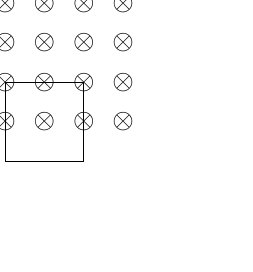
\begin{tikzpicture}
			\def\a{1};
			\def\l{2};
			\def\h{2};

			\foreach \x in {0,0.5,...,\l}
			{
				\foreach \y in {0,0.5,...,\h}
				{
					\node at (\x,\y) {$\otimes$};
				}
			}

			\draw (\l/2 - \a/2,-\a/2) rectangle (\l/2 + \a/2,\a/2);
		\end{tikzpicture}
	\end{figure}
	If the magnetic field is $1 \tesla$, find the terminal velocity of the loop in $\si{\metre\per\second}$.
	Find the velocity of the loop as a function of time.
	How long does it take, in seconds, to reach, say $90\%$ of the terminal velocity?
	What would happen is you cut a tiny slit in the ring?\\
	Note: The dimensions of the loop cancel out.
	Determine the actual numbers using the following values.
	\begin{itemize}
		\item Resistivity of aluminium: $\rho = 2.8 \times 10^{-8} \si{\ohm\metre}$
		\item Mass density of aluminium: $\eta = 2.7 \times 10^3 \si{\kg\per\metre\cubed}$
	\end{itemize}
\end{question}

\begin{solution}
	Let the length of the side of the loop be $l$.\\
	Let the cross-sectional area of the loop be $A$.\\
	Let the velocity of the loop be $v$.\\
	Therefore,
	\begin{align*}
		\varepsilon &= B l v\\
		\therefore I R &= B l v\\
		\therefore I &= \frac{B l v}{R}
	\end{align*}
	Therefore,
	\begin{align*}
		F_B &= I l B\\
		&= \frac{B l v}{R} l B\\
		&= \frac{B^2 l^2 v}{R}\\
		&= \frac{B^2 l^2 v}{4 \frac{\rho l}{A}}\\
		&= \frac{A B^2 l^2 v}{4 \rho l}
	\end{align*}
	When the loop reaches terminal velocity,
	\begin{align*}
		F_g &= F_B\\
		\therefore m g &= \frac{A B^2 l^2 v_t}{4 l \rho}\\
		\therefore v_t &= \frac{4 l \rho m g}{A B^2 l^2}\\
		&= \frac{4 l \rho (4 A l \eta) g }{A B^2 l^2}\\
		&= \frac{16 l^2 A \rho \eta g}{A B^2 l^2}\\
		&= \frac{16 \rho \eta g}{B^2}
	\end{align*}
	Therefore, as $B = 1 \tesla$, $\rho = 2.8 \times 10^{-8} \si{\ohm\metre}$, $\eta = 2.7 \times 10^3 \si{\kg\per\metre\cubed}$,\\
	\begin{align*}
		v &= \frac{(16) \left( 2.8 \times 10^{-8} \right) \left( 2.7 \times 10^3 \right) g}{1^2}\\
		&= (16) (2.8) (2.7) (g) \left( 10^{-5} \right)\\
		&= 120.96 g \times 10^{-5} \si{\metre\per\second}
	\end{align*}
	\begin{align*}
		\dod{v}{t} &= a\\
		&= g - \frac{A B^2 l^2 v}{4 m \rho l}\\
		&= g - \frac{A B^2 l^2 v}{4 (4 A l \eta) \rho l}\\
		&= g - \frac{A B^2 l^2 v}{ 16 A l^2 \rho \eta}\\
		&= g - \frac{B^2 v}{16 \rho \eta}\\
		\therefore \frac{\dif v}{g - \frac{B^2 v}{16 \rho \eta}} &= \dif t\\
		\therefore \int\limits_{0}^{v} \frac{\dif v}{g - \frac{B^2 v}{16 \rho \eta}} &= \int\limits_{0}^{t} \dif t
	\end{align*}
	Therefore, integrating,
	\begin{align*}
		\therefore -\frac{16 \rho \eta}{B^2} \left( \ln\left( g - \frac{B^2 v}{16 \rho \eta} \right) - \ln g \right) &= t\\
		\therefore \ln\left( \frac{g - \frac{B^2 v}{16 \rho \eta}}{g} \right) &= -\frac{B^2 t}{16 \rho \eta}\\
		\therefore \frac{g - \frac{B^2 v}{16 \rho \eta}}{g} &= e^{-\frac{B^2 t}{16 \rho \eta}}\\
		\therefore \frac{B^2 v}{16 \rho \eta} &= g - g e^{-\frac{B^2 t}{16 \rho \eta}}\\
		\therefore v &= \frac{16 \rho \eta g}{B^2} \left( 1 - e^{-\frac{B^2 t}{16 \rho \eta}} \right)\\
		&= v_t \left( 1 - e^{-\frac{B^2 t}{16 \rho \eta}} \right)
	\end{align*}
	Therefore, if $v = 0.9 v_t$,
	\begin{align*}
		0.9 v_t &= v_t \left( 1 - e^{-\frac{B^2 t}{16 \rho \eta}} \right)\\
		\therefore 0.9 &= 1 - e^{-\frac{B^2 t}{16 \rho \eta}}\\
		\therefore e^{-\frac{B^2 t}{16 \rho \eta}} &= 0.1\\
		\therefore -\frac{B^2 t}{16 \rho \eta} &= \ln 0.1\\
		\therefore t &= -\frac{16 \rho \eta \ln(0.1)}{B^2}
	\end{align*}
	If a tiny slit is cut in the ring, there will be no current flowing in the ring.\\
	Therefore, there will will be no resisting force.\\
	Hence, the ring will fall under gravity only.
\end{solution}

\section{Inductors}

\begin{definition}[Self inductance]
	\begin{align*}
		L &= \frac{\varepsilon}{\dod{I}{t}}
	\end{align*}
	is called self inductance.
\end{definition}

\subsection{Energy Stored in an Inductor}

\begin{theorem}
	\begin{align*}
		U_L &= \frac{1}{2} L I^2
	\end{align*}
\end{theorem}

\subsection{Energy Density}

\begin{theorem}
	\begin{align*}
		u_L &= \frac{B^2}{2 \mu_0}
	\end{align*}
\end{theorem}

\subsection{Mutual Inductance}

\begin{definition}[Mutual Inductance]
	Consider two loops, loop $1$ and loop $2$.\\
	Let there be a current $I_1$ in loop $1$.\\
	Therefore, a magnetic field $B_1$ will be induced.\\
	Therefore, there will be a magnetic flux, ${\Phi_{B}}_{2 1}$, due to $B_1$, in loop $2$.\\
	As a result, there will be a potential difference, $\varepsilon_2$, induced in loop $2$.
	Hence, there will be a current, $I_2$, induced in loop $2$.\\
	The mutual inductance of the two loops is defined as
	\begin{align*}
		\varepsilon_2 &= -M_{2 1} \dot{I_1}
	\end{align*}
	\begin{equation*}
		M_{1 2} = M_{2 1} = M
	\end{equation*}
\end{definition}

\section{Transformers}

\begin{theorem}
	\begin{align*}
		\frac{\varepsilon_1}{n_1} & = \frac{\varepsilon_2}{n_2}
	\end{align*}
\end{theorem}

\section{Maxwell's Correction to Ampere's Law}

\begin{definition}[Displacement current density]
	\begin{align*}
		\overrightarrow{j_D} & = \varepsilon_0 \dpd{\overrightarrow{E}}{t}
	\end{align*}
	is called the displacement current density.
\end{definition}

\begin{law}[Maxwell's Correction to Ampere's Law]
	\begin{align*}
		\overrightarrow{\nabla} \times \overrightarrow{B} & = \mu_0 \overrightarrow{j} + \mu_0 \varepsilon_0 \dpd{\overrightarrow{E}}{t} \\
                                                                  & = \mu_0 \overrightarrow{j} + \mu_0 \overrightarrow{j_D}
	\end{align*}
	Therefore,
	\begin{align*}
		\oint\limits_{\partial S} \overrightarrow{B} \cdot \overrightarrow{\dif l} & = \mu_0 \iint\limits_{S} \overrightarrow{j} \cdot \overrightarrow{\dif A} + \mu_0 \varepsilon_0 \dod{}{t}\iint\limits_{S} \overrightarrow{E} \cdot \overrightarrow{\dif A} \\
                                                                                           & = \mu_0 I \cdot \overrightarrow{\dif A} + \mu_0 I_D
	\end{align*}
	\label{Maxwell's_Correction_to_Ampere's_Law}
\end{law}

\begin{question}
	A capacitor has circular plates of radius $a$ with distance $d$ between them.\\
	It is connected by wires with distance $L$ between the wires.\\
	A rod is kept connecting the wires, as shown.\\
	A constant magnetic field $B$ is directed inwards as shown.
	\begin{figure}[H]
		\begin{tikzpicture}
			\def\a{0.5};
			\def\d{1};
			\def\L{3};
			\def\F{1};
			
			\coordinate (bottom plate centre) at (0,-\d/2);
			\coordinate (top plate centre) at (0,\d/2);
			
			\begin{scope}
				\clip (\L/2,-\L/2) rectangle (2*\L,\L/2);
				\foreach \x in {0,...,10}
				{
					\foreach \y in {-10,...,10}
					{
						\node at (\x,\y) {$\otimes$};
					}
				}
			\end{scope}

			\begin{scope}[ultra thick]
				\draw ($ (bottom plate centre) + (-\a,0) $) -- ($ (bottom plate centre) + (\a,0) $);
				\draw ($ (top plate centre) + (-\a,0) $) -- ($ (top plate centre) + (\a,0) $);
			\end{scope}

			\begin{scope}
				\draw (bottom plate centre) -- (0,-\L/2);
				\draw (top plate centre) -- (0,\L/2);

				\draw (0,-\L/2) -- (2*\L,-\L/2);
				\draw (0,\L/2) -- (2*\L,\L/2);
			\end{scope}

			\begin{scope}[ultra thick]
				\draw (\L,\L/2) -- (\L,-\L/2);
			\end{scope}

			\begin{scope}
				\draw [-stealth] (\L,0) -- ++(\F,0) node [right] {$v$};
			\end{scope}
		\end{tikzpicture}
	\end{figure}
	The rod is moving to the right with $v = \alpha t^2$.\\
	Find the magnetic field induced between the plates of the capacitor.
\end{question}

\begin{solution}
	As the rod is moving, there is an induced emf $\varepsilon$ between the ends of the rod.\\
	Therefore, the system is equivalent to
	\begin{figure}[H]
		\begin{circuitikz}
			\draw (0,0) to [C = $C$] (0,2);
			\draw (0,2) to (2,2);
			\draw (2,0) to [battery1 = $\varepsilon$] (2,2);
			\draw (2,0) to (0,0);
		\end{circuitikz}
	\end{figure}
	Therefore,
	\begin{align*}
		C           & = \frac{A \varepsilon_0}{d}       \\
                            & = \varepsilon_0 \frac{\pi a^2}{d} \\
		\varepsilon & = v B L                           \\
                            & = \alpha t^2 B L
	\end{align*}
	Let the charge on the plates of the capacitor by $+Q$ and $-Q$.\\
	Therefore,
	\begin{align*}
		Q & = C \varepsilon \\
                  & = \varepsilon_0 \frac{\pi a^2}{d} \alpha t^2 B L
	\end{align*}
	The electric field between the capacitor plates is
	\begin{align*}
		E & = \frac{\varepsilon}{d} \\
                  & = \frac{\alpha t^2 B L}{d}
	\end{align*}
	Consider a virtual Ampereian loop of radius $r$, between the capacitor plates.\\
	Let this loop be directed clockwise if seen from above.\\
	Let the magnetic field acting on the loop be $\tilde{B}$.\\
	Therefore, by \nameref{Maxwell's_Correction_to_Ampere's_Law},
	\begin{align*}
		\oint \overrightarrow{B} \cdot \overrightarrow{\dif l} & = \cancelto{0}{\mu_0 \iint \overrightarrow{j} \cdot \dif \overrightarrow{A}} + \mu_0 \varepsilon_0 \dod{}{t}\iint \overrightarrow{E} \cdot \dif \overrightarrow{A} \\
                                                                       & = \mu_0 \varepsilon_0 \dod{}{t}\left( \frac{\alpha t^2 B L}{d} \pi r^2 \right)                                                                                     \\
		\therefore \tilde{B} \cdot 2 \pi r                     & = \mu_0 \varepsilon_0 \frac{2 \alpha t B L}{d} \pi r^2                                                                                                             \\
		\therefore \tilde{B}                                   & = \frac{\mu_0 \varepsilon_0 \alpha B L}{d} t r
	\end{align*}
	Therefore, as $\overrightarrow{\tilde{B}}$ is positive, it is directed parallel to $\dif l$.\\
	Therefore, it supports its cause.\\
	In general, the magnetic field induced due to a change in $\Phi_B$ opposes its own cause, and the magnetic field induced due to a change in $\Phi_E$ supports it own cause.
\end{solution}

\begin{question}
	A capacitor with circular plates of radius $a$ and distance $d$ between them is connected to a battery of voltage $V$.\\
	The capacitor is filled with a liquid dielectric of dielectric constant $\kappa$.\\
	The dielectric is leaking through the bottom, such that the level of the liquid is falling with velocity $u$, as shown.
	Find the magnetic field inside the capacitor and the displacement current.
	\begin{figure}[H]
		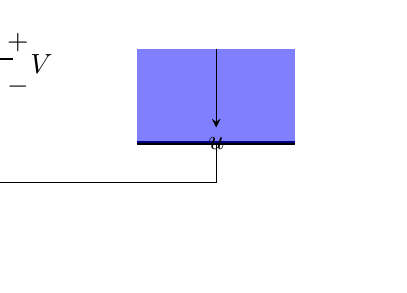
\begin{tikzpicture}
			\def\a{1};
			\def\d{2};
			\def\L{3};
			\def\F{1};
			\def\h{0.6*\d};

			\coordinate (bottom plate centre) at (3*\a,-\d/2);
			\coordinate (top plate centre) at (3*\a,\d/2);

			\begin{scope}[ultra thick]
				\draw ($ (bottom plate centre) + (-\a,0) $) -- ($ (bottom plate centre) + (\a,0) $);
				\draw ($ (top plate centre) + (-\a,0) $) -- ($ (top plate centre) + (\a,0) $);
			\end{scope}

			\begin{scope}
				\draw (bottom plate centre) -- (3*\a,-\L/2);
				\draw (top plate centre) -- (3*\a,\L/2);

				\draw (0,-\L/2) -- (3*\a,-\L/2);
				\draw (0,\L/2) -- (3*\a,\L/2);

				\draw (0,\L/2) to [battery1 = $V$] (0,-\L/2);
			\end{scope}
			\begin{scope}
				\fill [blue, opacity = 0.5] ($ (bottom plate centre) + (-\a,0) $) rectangle ($ (bottom plate centre) + (\a,\h) $);
				\draw [-stealth] ($ (bottom plate centre) + (0,\h) $) -- ++(-90:\F) node [below] {$u$};
			\end{scope}
		\end{tikzpicture}
	\end{figure}
\end{question}

\begin{solution}
	The capacitor is equivalent to a capacitor filled completely with the dielectric connected in series with a capacitor with a vacuum inside it.\\
	Therefore,
	\begin{align*}
		\frac{1}{C} & = \frac{1}{\varepsilon_0 \frac{A}{u t}} + \frac{1}{\varepsilon_0 \kappa \frac{A}{d - u t}}            \\
                            & = \frac{1}{\varepsilon_0 A} \left( \frac{1}{\frac{1}{u t}} + \frac{1}{\frac{\kappa}{d - u t}} \right) \\
                            & = \frac{1}{\varepsilon_0 A} \left( u t + \frac{d - u t}{\kappa} \right)                               \\
                            & = \frac{1}{\varepsilon_0 A} \left( \frac{d}{k} + u t \left( 1 - \frac{1}{k} \right) \right)
	\end{align*}
	Therefore,
	\begin{align*}
		C & = \varepsilon_0 \frac{A}{\frac{d}{k} + u t \left( \frac{k - 1}{k} \right)} \\
                  & = \varepsilon_0 \kappa \frac{A}{d + u t (\kappa - 1)}
	\end{align*}
	Therefore, the charge on the bottom plate of the capacitor is,
	\begin{align*}
		Q & = C V \\
                  & = \varepsilon_0 \kappa \frac{A V}{d + u t (\kappa + 1)}
	\end{align*}
	Let the electric field in the area of the capacitor which has vacuum be $E_{\textnormal{vacuum}}$.\\
	Let the electric field in the area of the capacitor which has dielectric be $E_{\textnormal{dielectric}}$.\\
	Let both $E_{\textnormal{vacuum}}$ and $E_{\textnormal{dielectric}}$ be directed from the bottom plate to the top plate, i.e. upwards.\\
	Therefore,
	\begin{align*}
		E_{\textnormal{dielectric}} & = \frac{\sigma}{\kappa \varepsilon_0} \\
                                            & = \frac{Q}{\kappa \varepsilon_0 A}    \\
                                            & = \frac{\kappa V}{\kappa \left( d + u t (\kappa - 1) \right)}
	\end{align*}
	Consider a box shaped Gaussian surface at the upper surface of the dielectric, with the bottom surface in the dielectric and the top surface in vacuum.\\
	Therefore, the electric field entering the surface is $\frac{\kappa V}{\kappa \left( d + u t (\kappa - 1) \right)}$, and the electric field exiting the surface is $\frac{\kappa V}{d + u t (\kappa + 1)}$.\\
	Therefore, by Gauss' Law,
	\begin{align*}
		\frac{\kappa V}{d + u t (\kappa - 1)} - \frac{\kappa V}{\kappa \left( d + u t (\kappa - 1) \right)} & = \frac{\sigma_{\textnormal{bound}}}{\varepsilon_0} \\
		\therefore \varepsilon_0 \left( \frac{\kappa V}{d + u t (\kappa - 1)} - \frac{V}{d + u t (\kappa - 1)} \right) &= \sigma_{\textnormal{bound}}
	\end{align*}
	Consider a virtual Ampereian loop of radius $r$ in the area of the capacitor with vacuum.\\
	Therefore, by \nameref{Maxwell's_Correction_to_Ampere's_Law},
	\begin{align*}
		\oint\limits_{\partial S} \overrightarrow{B} \cdot \overrightarrow{\dif l} & = \mu_0 \iint\limits_{S} \overrightarrow{j} \cdot \overrightarrow{\dif A} + \mu_0 \varepsilon_0 \dod{}{t} \iint\limits_{D} \overrightarrow{E} \cdot \dif \overrightarrow{A} \\
                                                                                           & = \mu_0 \varepsilon_0 \dod{}{t}\left( \frac{\kappa V}{d + u t (\kappa - 1)} \pi r^2 \right)                                                                                 \\
                                                                                           & = \mu_0 \varepsilon_0 \left( -\frac{\kappa V u (\kappa - 1)}{\left( d + u t (\kappa - 1) \right)^2} \pi r^2 \right)
	\end{align*}
	The charge on the bottom plate of the capacitor is,
	\begin{align*}
		Q              & = \varepsilon_0 \kappa \frac{A V}{d + u t (\kappa - 1)} \\
		\therefore Q_i & = \varepsilon_0 \frac{A V}{d + u \cdot 0 (\kappa - 1)}  \\
                               & = \varepsilon_0 \kappa \frac{A V}{d}                    \\
		\therefore Q_f & = \varepsilon_0 \frac{A V}{d + d (\kappa - 1)}          \\
                               & = \varepsilon_0 \frac{A V}{d}
	\end{align*}
	Therefore, the charge on the plate is reducing.
	Hence, the current in the circuit will be from the bottom plate to the top plate, i.e. clockwise.\\
	Therefore, the induced magnetic field inside the capacitor will be such that the magnetic field due to it is directed downwards.
	Therefore, it supports its own cause.\\
	This is consistent with the expectations.\\
	Therefore, the displacement current is,
	\begin{align*}
		I_D & = \frac{\oint\limits_{\partial S} \overrightarrow{B} \cdot \overrightarrow{\dif l}}{\mu_0} \\
                    & = \varepsilon_0 \dod{}{t}\left( \frac{\kappa V}{d + u t (\kappa - 1)} \pi r^2 \right)      \\
                    & = \varepsilon_0 \left( -\frac{\kappa V u (\kappa - 1)}{\left( d + u t (\kappa - 1) \right)^2} \pi r^2 \right)
	\end{align*}
\end{solution}

\begin{question}
	A capacitor with circular plates of radius $a$ and distance $d$ between them is filled with a material of conductivity $\sigma$.
	The capacitor connected to a sinusoidal voltage source $V = V_0 \sin \omega t$.
	Find the magnetic field induced inside the capacitor.
\end{question}

\begin{solution}
	Let the electric field inside the capacitor be $E$.
	Let $E$ be directed upwards, i.e. in the $\hat{z}$ direction.\\
	\begin{align*}
		\overrightarrow{E}            & = \frac{V}{d} \hat{z}                 \\
                                              & = \frac{V_0 \sin \omega t}{d} \hat{z} \\
		\therefore \overrightarrow{j} & = \sigma \overrightarrow{E}           \\
                                              & = \frac{\sigma V_0 \sin \omega t}{d} \hat{z}
	\end{align*}
	Consider a virtual Ampereian loop with radius $r$ inside the capacitor.\\
	Therefore, by \nameref{Maxwell's_Correction_to_Ampere's_Law},
	\begin{align*}
		\oint\limits_{\partial S} \overrightarrow{B} \cdot \overrightarrow{\dif l} & = \mu_0 \iint\limits_{S} \overrightarrow{j} \cdot \dif \overrightarrow{A} + \mu_0 \varepsilon_0 \dod{}{t}\iint\limits_{S} \overrightarrow{E} \cdot \dif \overrightarrow{A} \\
                                                                                           & = \mu_0 \frac{\sigma V_0 \sin \omega t}{d} \pi r^2 + \mu_0 \varepsilon_0 \dod{}{t}\left( \frac{V_0 \sin \omega t}{d} \pi r^2 \right)                                       \\
		\therefore 2 \pi r B                                                       & = \frac{V_0 \mu_0 \pi r^2}{d} \left( \sigma \sin \omega t + \varepsilon_0 \omega \cos \omega t \right)                                                                     \\
		\therefore B                                                               & = \frac{V_0 \mu_0 r}{2 d} (\sigma \sin \omega t + \varepsilon_0 \omega \cos \omega t)
	\end{align*}
\end{solution}

\end{spacing}

\end{multicols}

\section{Maxwell's Equations}

\doublespacing

\begin{tabular}{|l||l|l|}
	\hline
	Law                        & Integral Form                                                                                                                                                                                                                               & Differential Form                                                                                                                \\ [1.5ex]
	\hline
	Gauss' Law for Electricity & $\displaystyle \oiint\limits_{\partial V} \overrightarrow{E} \cdot \dif \overrightarrow{A} = \frac{1}{\varepsilon_0} \iiint\limits_{V} \rho \dif^3 r$                                                                                                                                       & $\overrightarrow{\nabla} \cdot \overrightarrow{E} = \frac{\rho}{\varepsilon_0}$                                                 \\ [1.5ex]

	Faraday's Law & $\displaystyle \oint\limits_{\partial S} \overrightarrow{E} \cdot \overrightarrow{\dif l} = -\dod{}{t} \iint\limits_{S} \overrightarrow{B} \cdot \dif \overrightarrow{A}$ & $\overrightarrow{\nabla} \times \overrightarrow{E} = -\dpd{\overrightarrow{B}}{t}$ \\ [1.5ex]

	Gauss' Law for Magnetism & $\displaystyle \oiint\limits_{S} \overrightarrow{B} \cdot \dif \overrightarrow{A} = 0$                                                                                                                                                      & $\overrightarrow{\nabla} \cdot \overrightarrow{B} = 0$                                                                           \\ [1.5ex]

	Ampere's Law               & $\displaystyle \overrightarrow{B} \cdot \overrightarrow{\dif l} = \mu_0 \iint\limits_{S} \overrightarrow{j} \cdot \dif \overrightarrow{A} + \mu_0 \varepsilon_0 \dod{}{t}\iint\limits_{S} \overrightarrow{E} \cdot \dif \overrightarrow{A}$ & $\overrightarrow{\nabla} \times \overrightarrow{B} = \mu_0 \overrightarrow{j} + \mu_0 \varepsilon_0 \dpd{\overrightarrow{E}}{t}$ \\ [1.5ex]

	\hline
\end{tabular}

\begin{multicols}{2}

\singlespacing

\end{multicols}

\end{document}
